\documentclass[14pt]{beamer}

\usetheme{Madrid}

% Add frame numbers
\setbeamertemplate{page number in head/foot}[framenumber]

\usepackage{amsmath, amssymb}
\usepackage{tikz}
\usepackage{bm}
\usepackage{outlines}   % For multilevel lists using the outline environment


\newcommand{\CMA}{Causal Mediation Analysis}
\newcommand{\bE}{\mathbb{E}}
\newcommand{\GLMMs}{Mixed-Effects Models}

\title[]{Statistical Considerations in Multilevel Mediation Analysis}
\author{William Ruth}
\institute[]{Collaborators: Rado Ramasy, Rowin Alfaro, Ariel Mundo, Bruno Remillard, Bouchra Nasri}
\date{\vspace{-3cm}}
\titlegraphic{
\includegraphics[width=2cm]{../Logos/CANSSI_Logo.png} \hspace{2cm} 
\includegraphics[width=4cm]{../Logos/Logo_UdeM-CMJN.jpg}}


\begin{document}

\begin{frame}
    \titlepage
\end{frame}

\begin{frame}{Outline}
    \begin{itemize}
        \setlength{\itemsep}{0.75em}
        \item[1)] The Problem
        \item[2)] Mediation Analysis
        \item[3)] Causal Inference
        \item[4)] Mixed-Effects Models
        \item[234)] Mixed-Effects Models in Causal Mediation Analysis
    \end{itemize}
\end{frame}

\begin{frame}{Example}
    \begin{itemize}
        \item Goal: Understand adherence to restrictive measures
        \begin{itemize}
            \item E.g. Lockdowns
            \item Both past and future \newline
        \end{itemize}
        \item Influence of news source
        \begin{itemize}
            \item How trustworthy? \newline
        \end{itemize}
        \item Disentangle influence on future from influence on past
    \end{itemize}
    
\end{frame}


\begin{frame}{Example}
        \begin{figure}[H]
            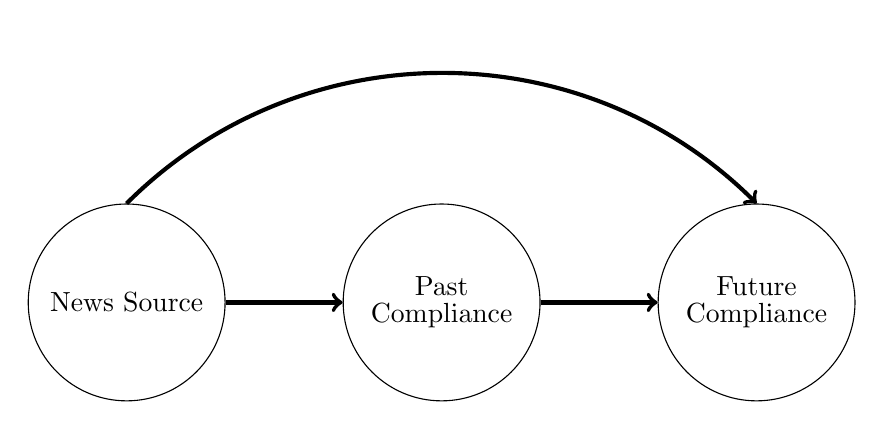
\begin{tikzpicture}
                % Circles with labels
                \node at (0,0) [circle, draw, minimum size=2.5cm] (news) {News Source};
                \node at (4,0) [circle, draw, minimum size=2.5cm] (past) {\shortstack{Past\\Compliance}};
                \node at (8,0) [circle, draw, minimum size=2.5cm] (future) {\shortstack{Future\\Compliance}};
                
                % Arrows
                \draw[->, line width=1.5pt] (news.east) -- (past.west);
                \draw[->, line width=1.5pt] (past.east) -- (future.west);
                \draw[->, line width=1.5pt, bend left] (news.north) to [out=45,in=135] (future.north); 
                
                \end{tikzpicture}
    \end{figure}
\end{frame}

\begin{frame}{Example}
    Terminology
    \begin{columns}
        \column{0.6\textwidth}
        \begin{itemize}
            \item Top path: {Direct effect}
            \item Center path: {Indirect effect}
            \item Combined: {Total effect}
        \end{itemize}
        \column{0.4\textwidth}
        \begin{itemize}
            \item Exposure: $X$
            \item Outcome: $Y$
            \item Mediator: $M$
        \end{itemize}
    \end{columns}
    
\end{frame}




\begin{frame}{Mediation Analysis}
    \begin{figure}[H]
        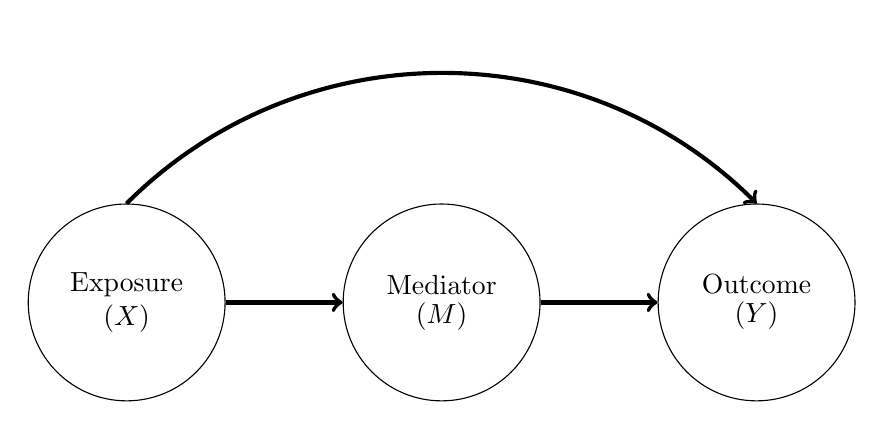
\begin{tikzpicture}
            % Circles with labels
            \node at (0,0) [circle, draw, minimum size=2.5cm] (X) {\shortstack{Exposure\\($X$)}};
            \node at (4,0) [circle, draw, minimum size=2.5cm] (M) {\shortstack{Mediator\\($M$)}};
            \node at (8,0) [circle, draw, minimum size=2.5cm] (Y) {\shortstack{Outcome\\($Y$)}};
            
            % Arrows
            \draw[->, line width=1.5pt] (X.east) -- (M.west);
            \draw[->, line width=1.5pt] (M.east) -- (Y.west);
            \draw[->, line width=1.5pt, bend left] (X.north) to [out=45,in=135] (Y.north); 
            
            \end{tikzpicture}
    \end{figure}
\end{frame}

\begin{frame}{Mediation Analysis}
    \begin{outline}
        \1 Separate \textbf{Total Effect} of $X$ on $Y$ into
            \2 \textbf{Direct Effect}
            \2 \textbf{Indirect Effect}\newline

        \1 Define mediation effects using counterfactuals
        \1 Differences, ratios, odds-ratios
    \end{outline}    
\end{frame}



\begin{frame}{Mediation Analysis}
    \begin{outline}
        \1 We only observe one outcome per individual\newline

        \1 Explore population-level effects by averaging\newline

        \1 Identify expected counterfactuals with conditional expectations
            \2 Now it's a regression problem
    \end{outline}
\end{frame}


\begin{frame}
    \frametitle{Mediation Analysis}
    \begin{outline}
        \1 Fit two regression models
            \2 Mediator given exposure
            \2 Outcome given mediator and exposure
            \2 Both may include confounders \newline

        \1 Linear vs Logistic
        \1 Fixed- vs Mixed-Effects
            \2 Single- vs Multi-Level
    \end{outline}
\end{frame}

\begin{frame}
    \frametitle{Mediation Analysis}
    \begin{outline}
        \1 Fit two regression models
            \2 Mediator given exposure
            \2 Outcome given mediator and exposure
            \2 Both may include confounders \newline

        \1 Linear vs \textbf{Logistic}
        \1 Fixed- vs \textbf{Mixed-Effects}
            \2 Single- vs Multi-Level
    \end{outline}
\end{frame}


\begin{frame}
    \frametitle{Mediation Analysis}
    \begin{outline}
        \1 Model fitting involves intractable integrals over unobserved random effects
            \2 Evaluate using quadrature 
        \1 Estimated mediation effects depend on coefficients and RE covariances\newline

        \1 Uncertainty quantification:
            \2 Quasi-Bayesian Monte Carlo
            \2 $\delta$-method
    \end{outline}
\end{frame}

\begin{frame}
    \frametitle{Uncertainty Quantification}
    \begin{outline}
        \1 Quasi-Bayesian Monte Carlo
            \2 Monte Carlo $\delta$-Method \newline
        \end{outline}

        \begin{enumerate}
            \item Estimate sampling distribution of regression parameters
            \item Simulate from estimated sampling distribution
            \item Compute mediation effects for simulated parameters
        \end{enumerate}
\end{frame}

\begin{frame}
    \frametitle{Uncertainty Quantification}
    \begin{outline}
        \1 Quasi-Bayesian Monte Carlo
            \2 Monte Carlo $\delta$-Method \newline

        \1 Advantage: Flexible        
        \1 Disadvantage: Computational \newline

        \1 Existing implementation in \texttt{R}: \textit{mediation}
            \2 Limited
        \end{outline}
\end{frame}




\begin{frame}
    \frametitle{Uncertainty Quantification}
    \begin{outline}
        \1 $\delta$-Method \newline
        \end{outline}

        \begin{enumerate}
            \item Estimate (asymptotic) sampling distribution of regression parameters
            \item Compute Jacobian of map from reg pars to mediation effects
            \item Multiply asymp. covariance by Jacobian
        \end{enumerate}
\end{frame}

\begin{frame}
    \frametitle{Uncertainty Quantification}
    \begin{outline}
        \1 $\delta$-Method \newline

        \1 Advantage: Analytical
        \1 Disadvantage: Asymptotic \newline

        \1 No existing \texttt{R} implementation
            \2 Until now!
            \2 Use \texttt{glmmTMB}, not \texttt{lme4}
        \end{outline}
\end{frame}


\begin{frame}
    \frametitle{Comparison}
    \begin{outline}
        \1 Simulate 200 datasets
            \2 \textbf{100} groups, \textbf{500} individuals per group \newline

        \1 Build confidence intervals using $\delta$- and MC $\delta$-methods \newline

        \1 Also build Wald interval using Monte Carlo (empirical) covariance matrix
        \end{outline}
\end{frame}

\begin{frame}
    \frametitle{Comparison}
    \begin{table}[h!]
        \centering
        \begin{tabular}{|cc|ccc|}
            \hline
            Effect & Scale & $\delta$ & MC $\delta$ & Empirical\\
            \hline
            Total & Diff & 0.940 & 0.940 & 0.940 \\
            & Ratio & 0.935 & 0.930& 0.955 \\
            & OR & 0.955 & 0.960 & 0.950 \\ 
            \hline
            Direct & Diff & 0.960 & 0.960 & 0.960 \\
            & Ratio & 0.935 & 0.930& 0.945 \\
            & OR & 0.970 & 0.970 & 0.950 \\
            \hline
            Indirect & Diff & 0.950 & 0.955 & 0.965 \\
            & Ratio & 0.955 & 0.955& 0.960 \\
            & OR & 0.955 & 0.955 & 0.960 \\
            \hline
        \end{tabular}
    \end{table}
\end{frame}

\begin{frame}
    \frametitle{Comparison}
    \begin{outline}
        \1 Simulate 200 datasets
            \2 \textbf{10} groups, \textbf{1000} individuals per group \newline

        \1 Build confidence intervals using $\delta$- and MC $\delta$-methods \newline

        \1 Also build Wald interval using Monte Carlo (empirical) covariance matrix

        \end{outline}
\end{frame}



\begin{frame}
    \frametitle{Comparison}
    \begin{table}[h!]
        \centering
        \begin{tabular}{|cc|ccc|}
            \hline
            Effect & Scale & $\delta$ & MC $\delta$ & Empirical\\
            \hline
            Total & Diff & 0.935 & 0.928 & 0.954 \\
            & Ratio & 0.961 & 0.974 & 0.967 \\
            & OR & 0.935 & 0.928 & 0.967 \\ 
            \hline
            Direct & Diff & 0.948 & 0.928 & 0.941 \\
            & Ratio & 0.928 & 0.935 & 0.967 \\
            & OR & 0.954 & 0.935 & 0.948 \\
            \hline
            Indirect & Diff & 0.974 & 0.967 & 0.961 \\
            & Ratio & 0.980 & 0.974 & 0.961 \\
            & OR & 0.948 & 0.928 & 0.948 \\
            \hline
        \end{tabular}
    \end{table}
\end{frame}



\begin{frame}
    \frametitle{Trust Study}
    \begin{outline}
        \1 Applying our method to the trust study dataset
            \2 Compare low-high trustworthiness \newline

        \1 CIs for all effect-scale pairs
            \2 9 Intervals \newline

        \1 $\delta$ and MC $\delta$
    \end{outline}
\end{frame}

\begin{frame}
    \frametitle{Trust Study}
    \centering
    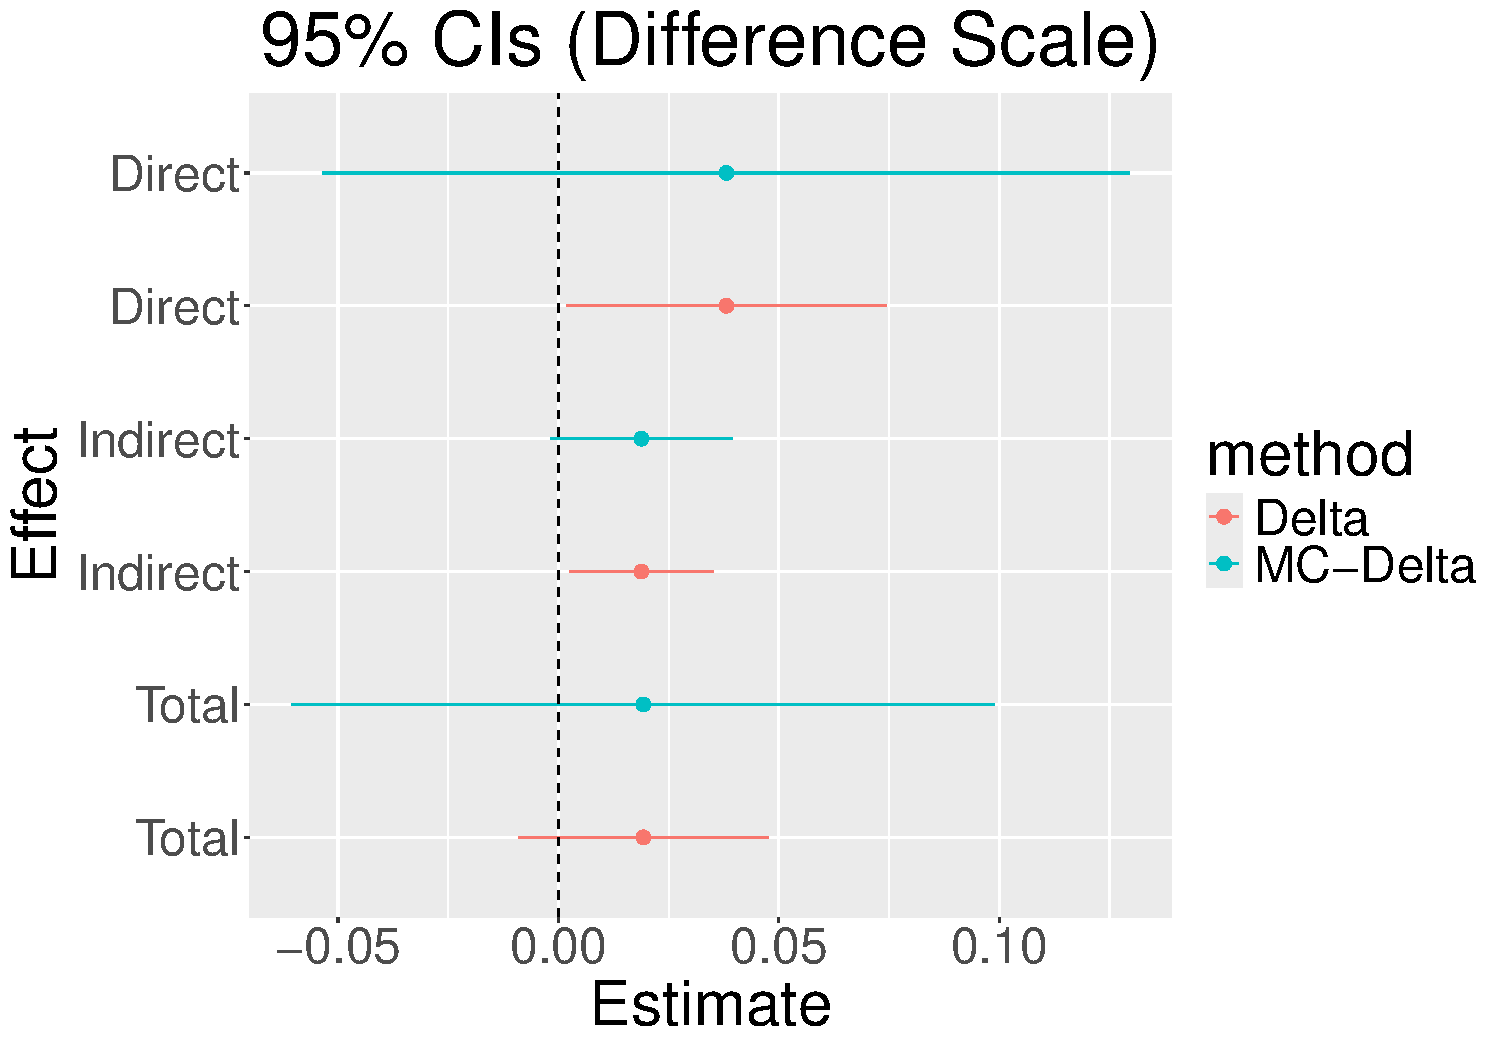
\includegraphics[height=0.9\textheight, width=0.9\textwidth, keepaspectratio]{Plots/CI_Plot-diff.pdf}
\end{frame}

\begin{frame}
    \frametitle{Trust Study}
    \centering
    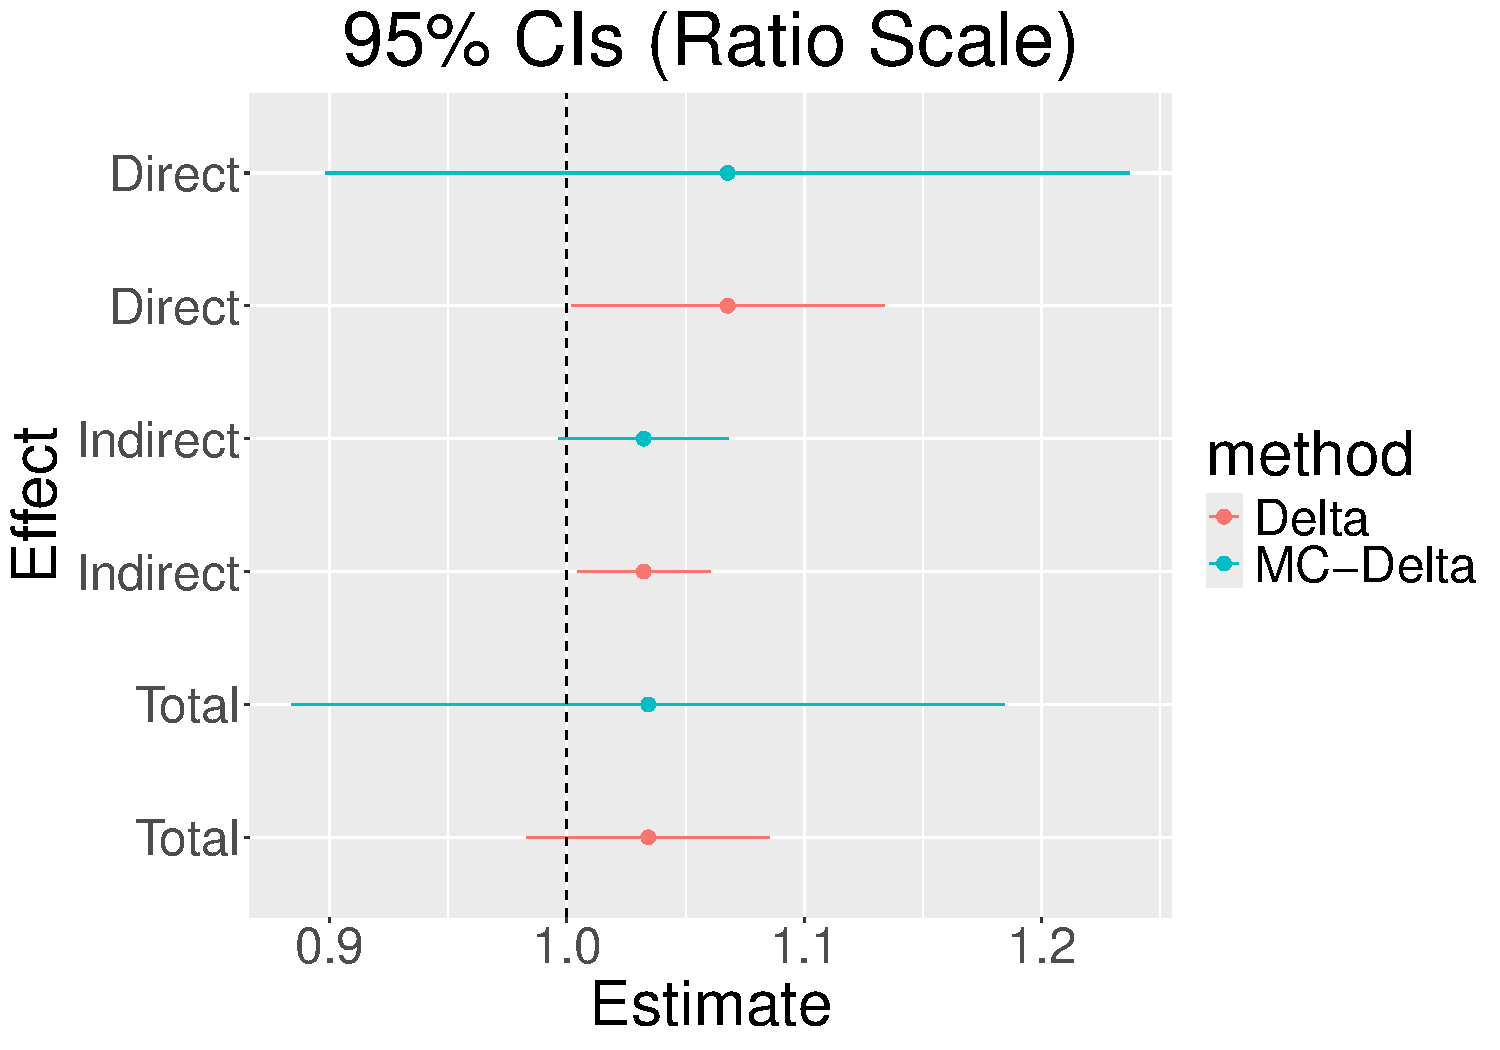
\includegraphics[height=0.9\textheight, width=0.9\textwidth, keepaspectratio]{Plots/CI_Plot-rat.pdf}
\end{frame}

\begin{frame}
    \frametitle{Trust Study}
    \centering
    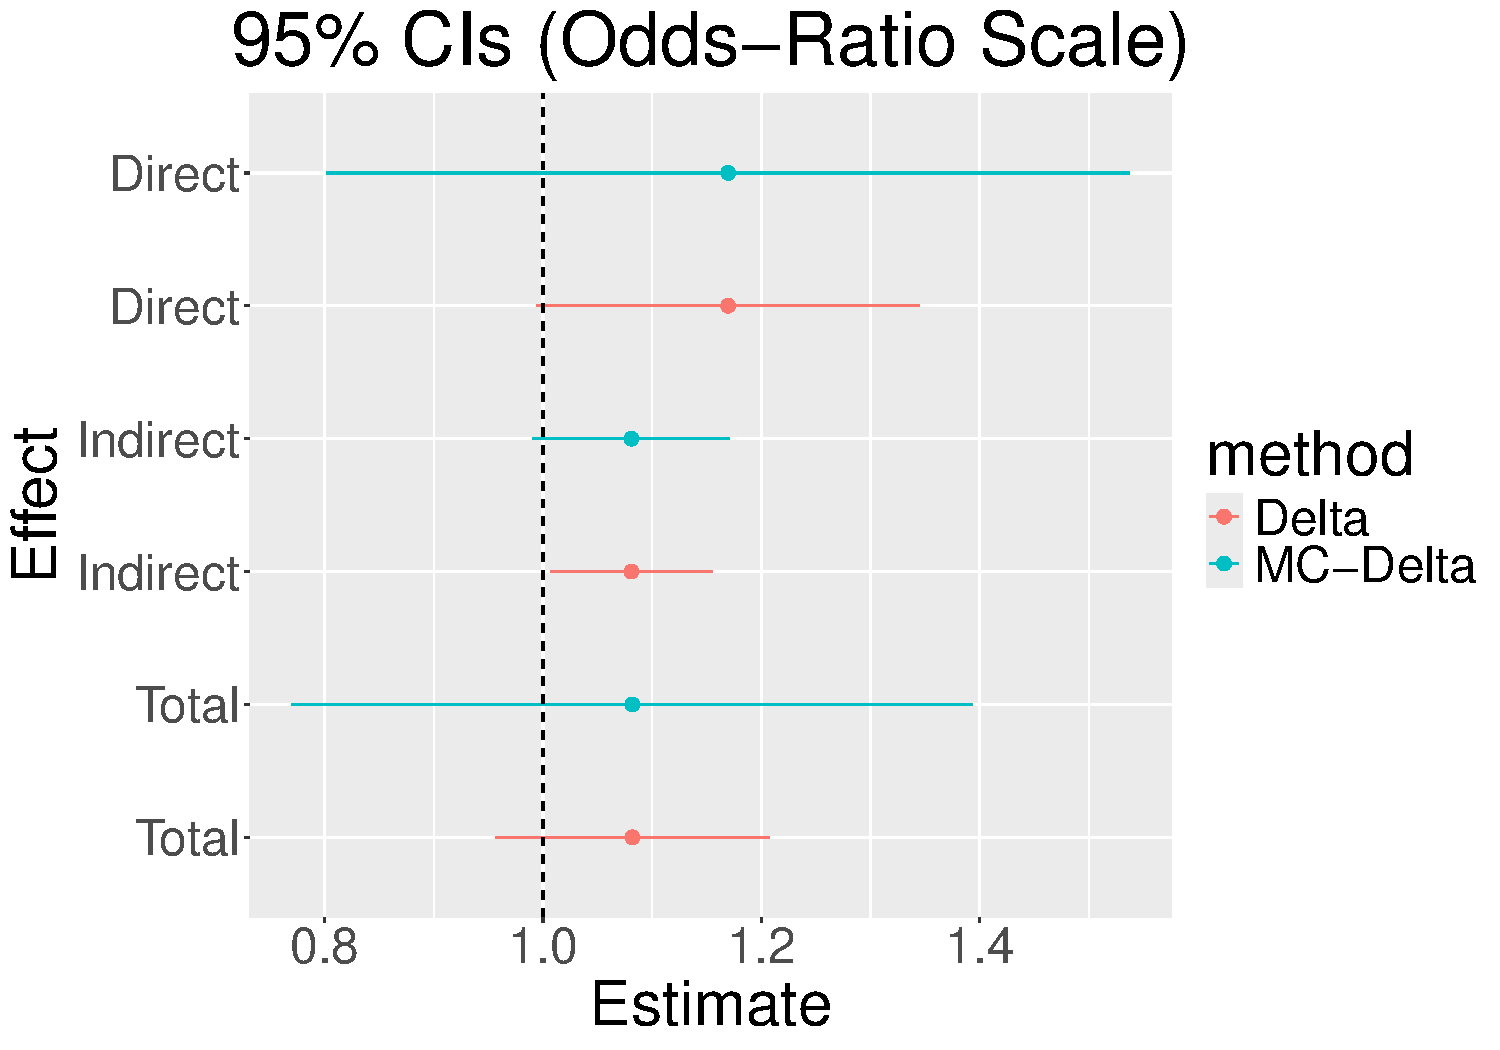
\includegraphics[height=0.9\textheight, width=0.9\textwidth, keepaspectratio]{Plots/CI_Plot-OR.pdf}
\end{frame}


\begin{frame}
    \frametitle{Next Steps}
    \begin{outline}
        \1 Compare with Imai et al. (\textit{mediation} package)

        \1 Sensitivity to values of confounders

        \1 Parametric bootstrap
        
        \1 Group-specific effects 
    \end{outline}
\end{frame}

\begin{frame}{Acknowledgements}
    Collaborators:
    \begin{itemize}
        \item Rado Ramasy
        \item Rowin Alfaro
        \item Ariel Mundo
        \item Bruno Remillard
        \item Bouchra Nasri \newline
    \end{itemize}

    Funding:
    \begin{itemize}
        \item Canadian Statistical Sciences Institute
    \end{itemize}
\end{frame}

\begin{frame}
    \centering
    \Huge Thank You
\end{frame}

\end{document}
